\documentclass{beamer}
\usepackage[utf8]{inputenc}
\usepackage{physics}
\usepackage[english,greek]{babel}
\usepackage{alphabeta}
\usepackage{amsmath, amssymb, amsfonts}
\usepackage{tikz, caption, subfig, comment, multicol, xcolor, tikz-feynman, tensor, graphics, graphicx, slashed, xfrac, biblatex, braket, siunitx, multirow, multicol}

\usefonttheme[onlymath]{serif}
% \setsansfont{TeX Gyre Termes}

\addbibresource{references.bib}
\usetheme{Madrid}
\usecolortheme{default}


\title[\href{https://summerstudent.web.cern.ch/home}{CERN Summer Student Programme 2023}]
{     
      New kinematic weighting algorithm for CP asymmetries in charm decays
}
\setbeamerfont{footnote}{size=\tiny}
\setbeamerfont{caption}{size=\tiny}

\author[\href{https://github.com/GiorgosChr}{Georgios Christou}]
{Georgios Christou
\\
Supervisors: Dr.\@ Federico Betti and Prof.\@ Angelo Carbone}

\institute[\href{https://lhcb.web.cern.ch/}{LHCb}]
{
      LHCb Collaboration
}

\date{August 29, 2023}

% \logo{
\includegraphics[height=0.7cm]{../.images/Lhcb-logo-new.svg.png}}
\logo{\href{https://lhcb.web.cern.ch/}{
\includegraphics[height=0.7cm]{../.images/Lhcb-logo-new.svg.png}}}


\AtBeginSection[]{
  \begin{frame}
    \tableofcontents[currentsection]
  \end{frame}
}


\begin{document}
\selectlanguage{english}
\frame{\titlepage}
\begin{frame}
      \tableofcontents
\end{frame}

\section{Introduction}
\subsection{Asymmetries at the LHCb}

\begin{frame}
      \frametitle{\insertsubsectionhead}
      \rightarrow We study CP asymmetries in the following charm decays
      \begin{eqnarray*}
            &D^{\star+}\to D^0\pi^+ \text{ and } D^{\star-}\to \bar{D}^0\pi^-, \nonumber\\
            &D^0 \to K^-K^+ \text{ and } D^0 \to \pi^-\pi^+
    \end{eqnarray*}
      \textbf{At LHCb we observe:}
      \begin{itemize}
            \item CP asymmetry \rightarrow Differences in matter and anti-matter decays
            \item Production asymmetry \rightarrow Differences in $D^{\star\pm}$ production
            \item Detection asymmetry \rightarrow Differences in $\pi_s^{\pm}$ detection
      \end{itemize}
      \bigbreak
      \rightarrow We mainly focus on CP and detection asymmetries throughout this project
\end{frame}

\begin{frame}
      \frametitle{\insertsubsectionhead}
      \rightarrow At an experiment our physical observable is the total asymmetry
      \begin{eqnarray*}
            &A_\text{total} = \frac{A_{CP} + A_{D}}{1 + A_{CP}A_D}\approx A_{CP} + A_{D} + \mathcal{O}(10^{-6}),\nonumber\\
            &A_{D} = \frac{\int \dd \vec{p} N(\vec{p})A(\vec{p})}{\int \dd \vec{p} N(\vec{p})}\to \text{ Integrated detection asymmetry}
      \end{eqnarray*}
      \rightarrow We can estimate the total asymmetry through
      \begin{equation*}
            A_\text{total} = \frac{N_+ - N_-}{N_+ + N_-}
      \end{equation*}
\end{frame}

\begin{frame}
      \frametitle{\insertsubsectionhead}
      \rightarrow We define the total asymmetry difference
      \begin{equation*}
            \Delta A_\text{total} = A_\text{total}^{KK} - A_\text{total}^{\pi\pi} = \Delta A_{CP} + \Delta A_{D}
      \end{equation*}

      \textbf{How can we calculate $\Delta A_{CP}$?}
      \begin{itemize}
            \item We can equalize $D^0$ kinematic distributions for $D^0\to K^-K^+$ and $D^0\to \pi^-\pi^+$ decay modes
            \item The following weighting function allows us to do that
      \end{itemize}
      \begin{equation*}
            Q(\vec{p}_{D^\star}, \vec{p}_{\pi_s}) \simeq \frac{\Gamma_{D^0}^{\pi\pi}(\vec{p}_{D^\star} - \vec{p}_{\pi_s}) + \Gamma_{\bar{D}^0}^{\pi\pi}(\vec{p}_{D^\star} - \vec{p}_{\pi_s})}{\Gamma_{D^0}^{KK}(\vec{p}_{D^\star} - \vec{p}_{\pi_s}) + \Gamma_{\bar{D}^0}^{KK}(\vec{p}_{D^\star} - \vec{p}_{\pi_s})}
      \end{equation*}
      \bigbreak
      \to The association with $\pi_s$ includes detection asymmetry to the weighting function $\Rightarrow$ {\bf We introduce bias!}
\end{frame}

\begin{frame}
      \frametitle{\insertsubsectionhead}
      \rightarrow We introduce a new weighting technique
      \begin{equation*}
            Q(\vec{p}_{D^0}) \simeq \frac{\Gamma_{D^0}^{\pi\pi}(\vec{p}_{D^0}) + \Gamma_{\bar{D}^0}^{\pi\pi}(\vec{p}_{D^0})}{\Gamma_{D^0}^{KK}(\vec{p}_{D^0}) + \Gamma_{\bar{D}^0}^{KK}(\vec{p}_{D^0})}\to \text{We eliminate the detection asymmetry}
      \end{equation*}
      \rightarrow We effectively equalize the distributions $\Rightarrow \Delta A_D = 0$
      \bigbreak
      \rightarrow Now our physical observable can give us useful results!
      \begin{equation*}
            \boxed{\Delta A_\text{total} = \Delta A_{CP}}
      \end{equation*}
      \bigbreak 
      {\bf However:}
      \begin{itemize}
            \item Such candidates were discarded in Run-2
            \item We do not have enough statistics from Run-3
      \end{itemize}
      \rightarrow We resort to MC data to test the new weighting technique
\end{frame}

\section{Analysis}
\subsection{RapidSim}

\begin{frame}
      \frametitle{\insertsubsectionhead}
      \rightarrow We generate data using RapidSim and introduce:
      \begin{itemize}
            \item Different CP asymmetries for $D^0\to K^-K^+$ and $D^0\to\pi^-\pi^+$ decay modes $\left(A_{CP}^{KK} = 0.1,\; A_{CP}^{\pi\pi} = 0.2,\; \rightarrow \Delta A_\text{total} = -0.1\right)$
            \item The same momentum-dependent detection asymmetry $A_D(\vec{p})$ \\ \rightarrow The integrated detection asymmetries are different for the two samples
      \end{itemize}
      \rightarrow We exclude negative $\pi_s$ \Rightarrow Large detection asymmetry
      \begin{figure}
            \centering
            \subfloat{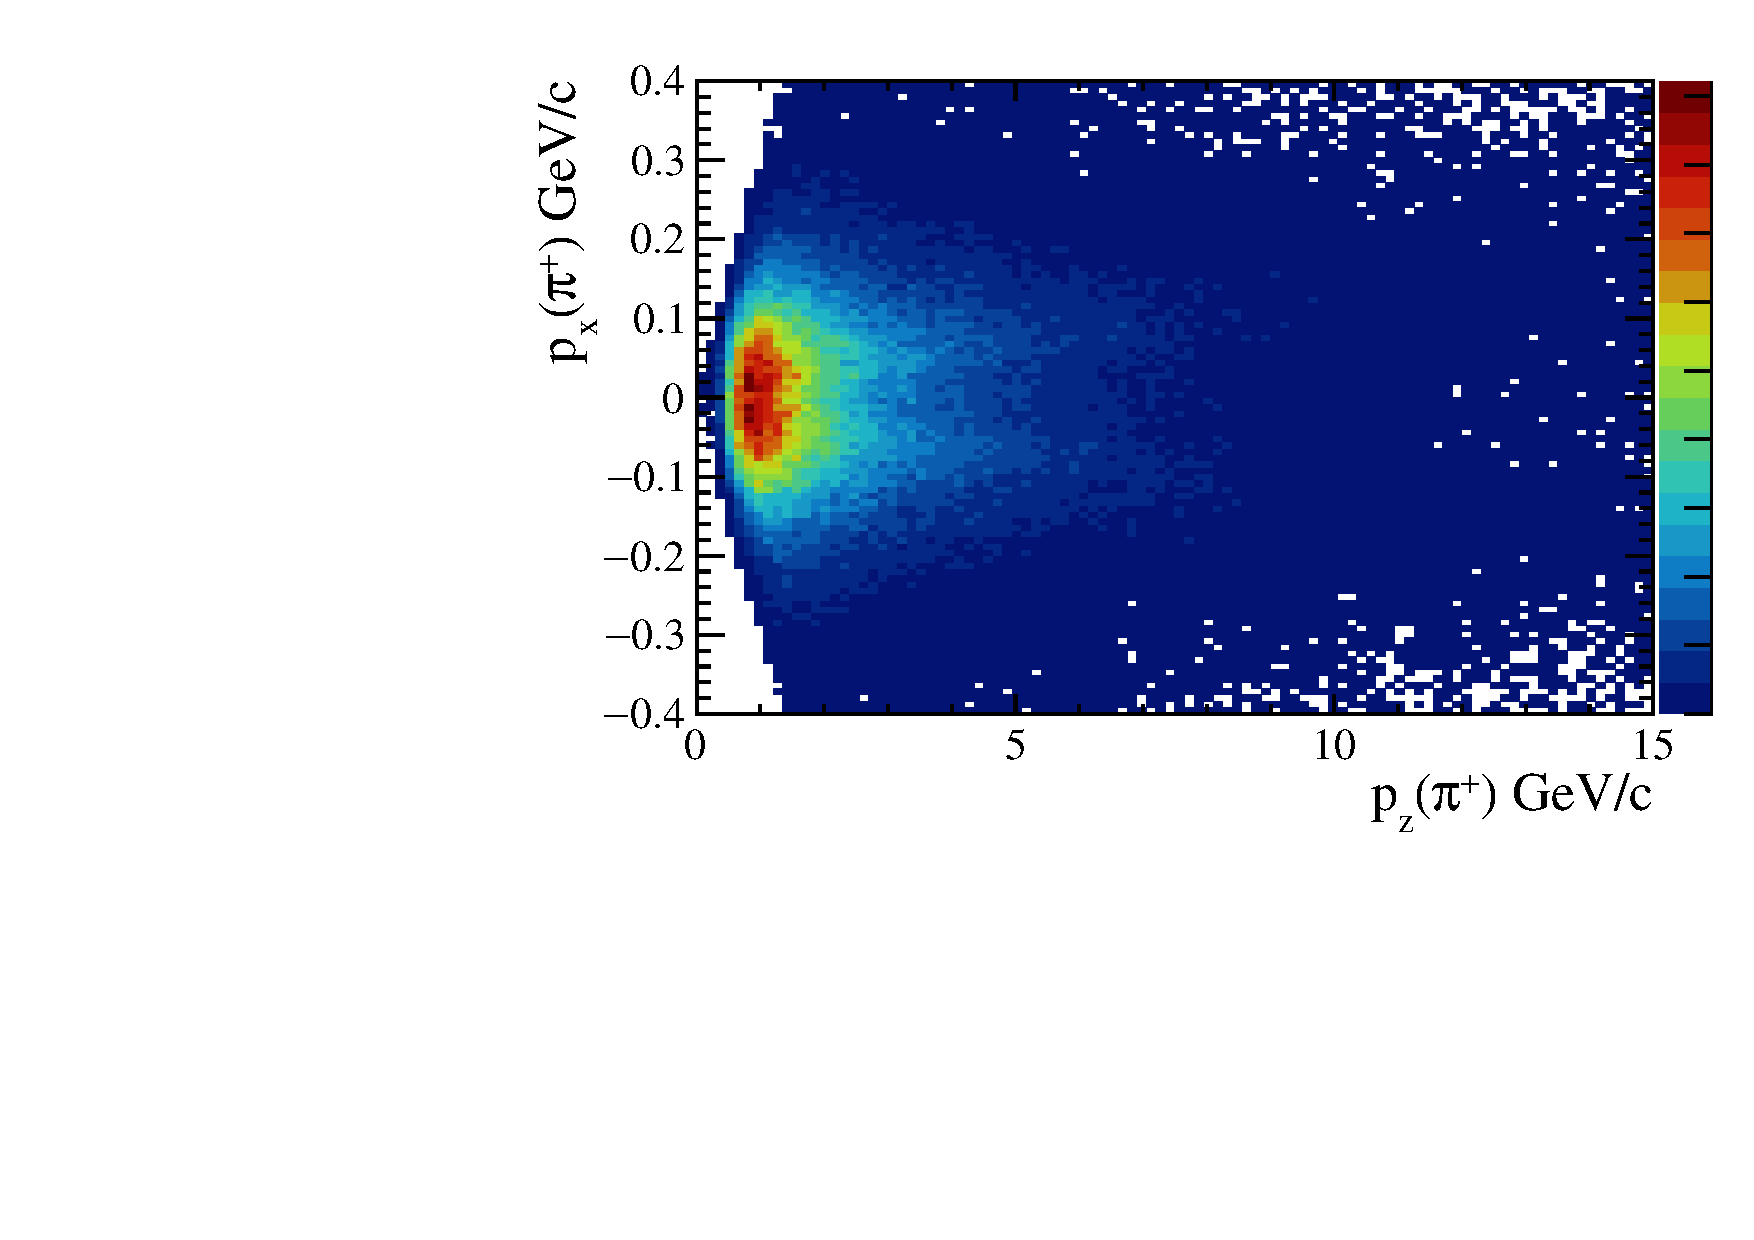
\includegraphics[width = 0.42\textwidth]{../work/RapidSimAnalysis/MomentumDependence/Plots/KK_Dst_PXPZ_Positive.pdf}}
            \subfloat{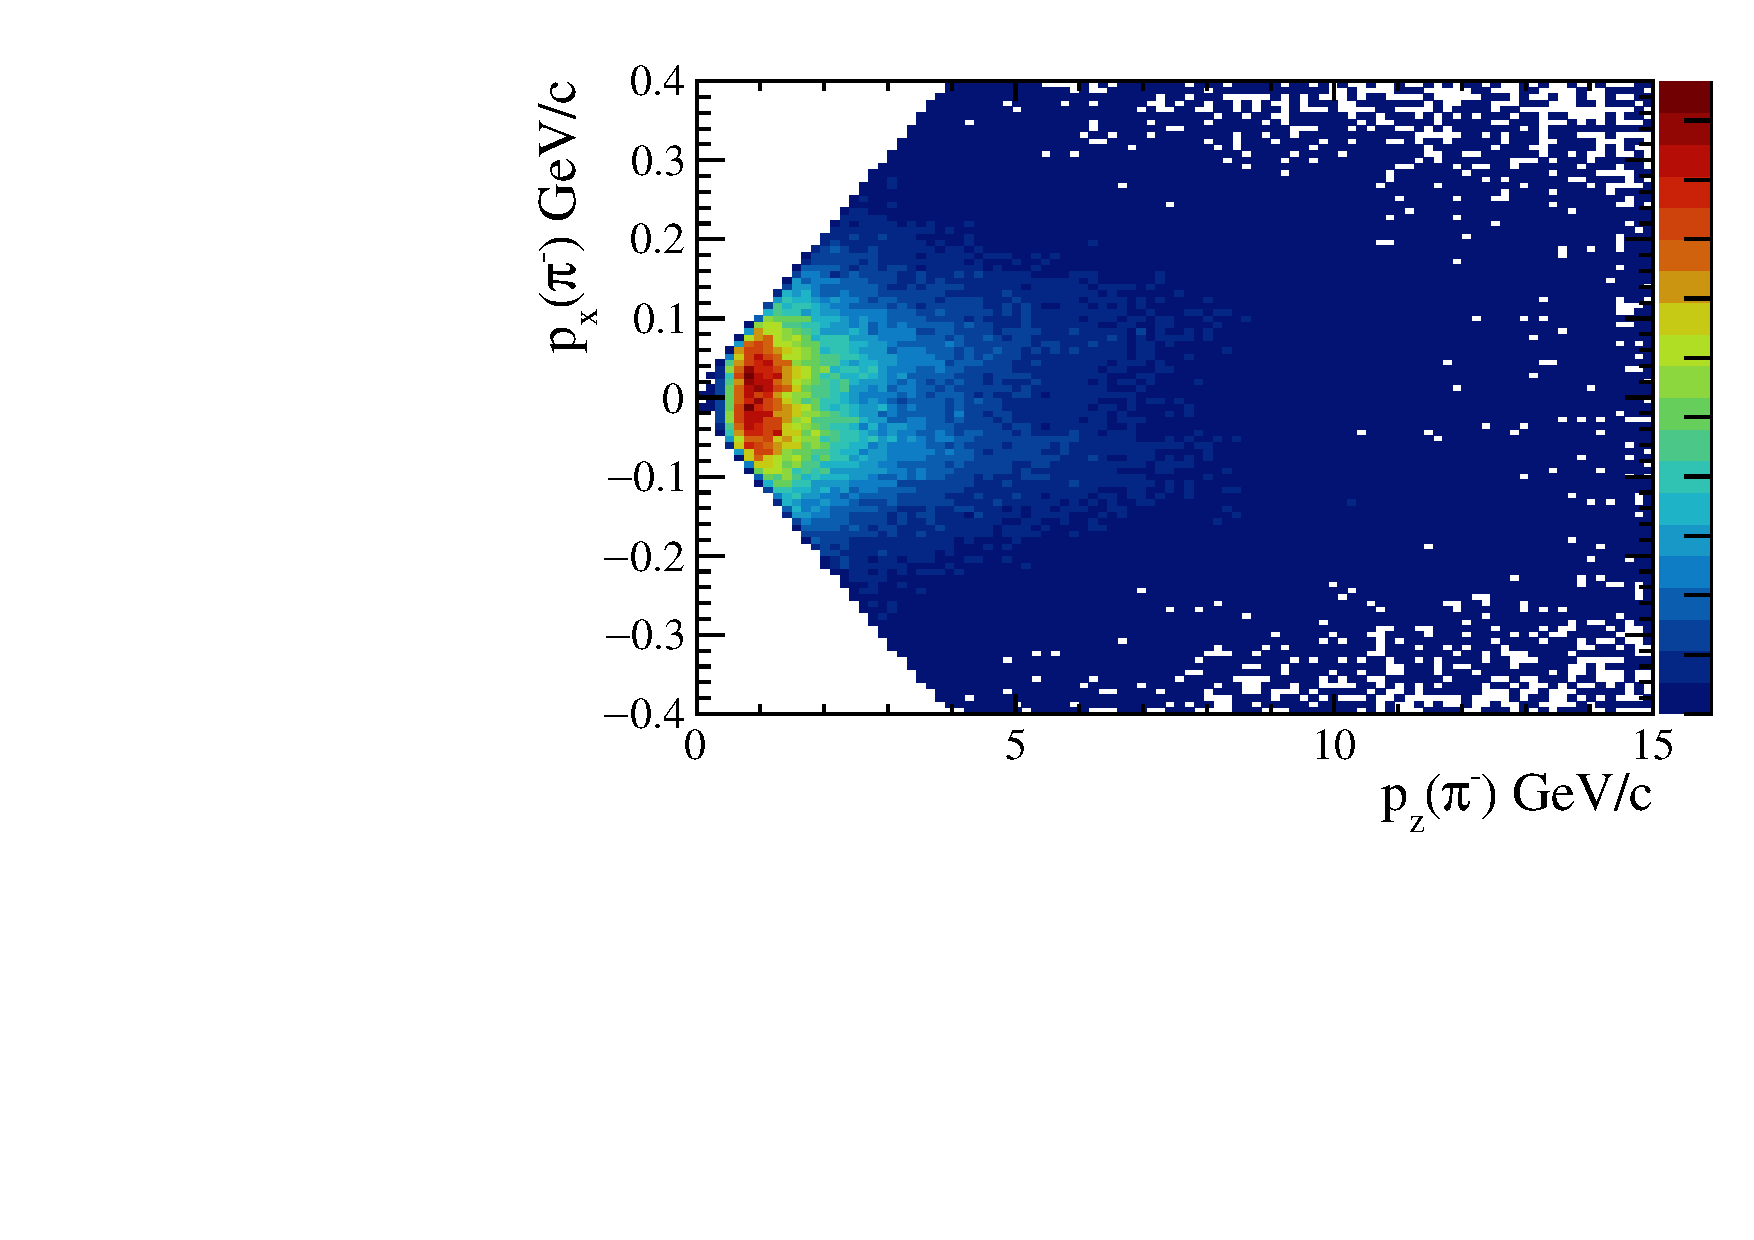
\includegraphics[width = 0.42\textwidth]{../work/RapidSimAnalysis/MomentumDependence/Plots/KK_Dst_PXPZ_Negative.pdf}}
      \end{figure}
\end{frame}

\begin{frame}
      \frametitle{\insertsubsectionhead}
      \rightarrow We calculate the weighting function before and after the introduction of the detection asymmetry
      \begin{itemize}
            \item Before: Not associated with $\pi_s$ \Rightarrow New weighting technique
            \item After: Associated with $\pi_s$ \Rightarrow We introduce bias
      \end{itemize}
      \begin{center}
            \scriptsize
            \begin{tabular}{c|c|c|c}
                  Technique& & Weighted & Unweighted\\
                  \hline\hline
                  \multirow{2}{*}{Not associated} & $\Delta A_\text{total}$ & $-0.09845 \pm 0.00094$ & \\
                  & Deviation $(\sigma)$ & $1.65$ & $-0.08303 \pm 0.00093$\\
                  \cline{1-3}
                  \multirow{2}{*}{Associated with $\pi_s$} & $\Delta A_\text{total}$ & $-0.09578 \pm 0.00094$ & $18.2$\\
                  & Deviation $(\sigma)$ & $4.49$ & \\
            \end{tabular}
    \end{center}
    \normalsize
    \begin{itemize}
      \item The unweighted calculation is wrong \rightarrow $\Delta A_D \neq 0$
      \item The weighting function with $\pi_s$ association (i.e., with detection asymmetry included) yields a biased result
      \item The new weighting technique (no detection asymmetry) allows us to keep events associated with large $A_D(\vec{p})$ \Rightarrow {\bf More statistics!}
    \end{itemize}
\end{frame}

\subsection{Particle Gun}

\begin{frame}
      \frametitle{\insertsubsectionhead}
      \rightarrow We use Particle Gun data for a more realistic scenario.
      \begin{itemize}
            \item We do not introduce CP asymmetry
            \item There is detection asymmetry due to the magnet polarity
      \end{itemize}
      \begin{figure}
            \centering
            \subfloat{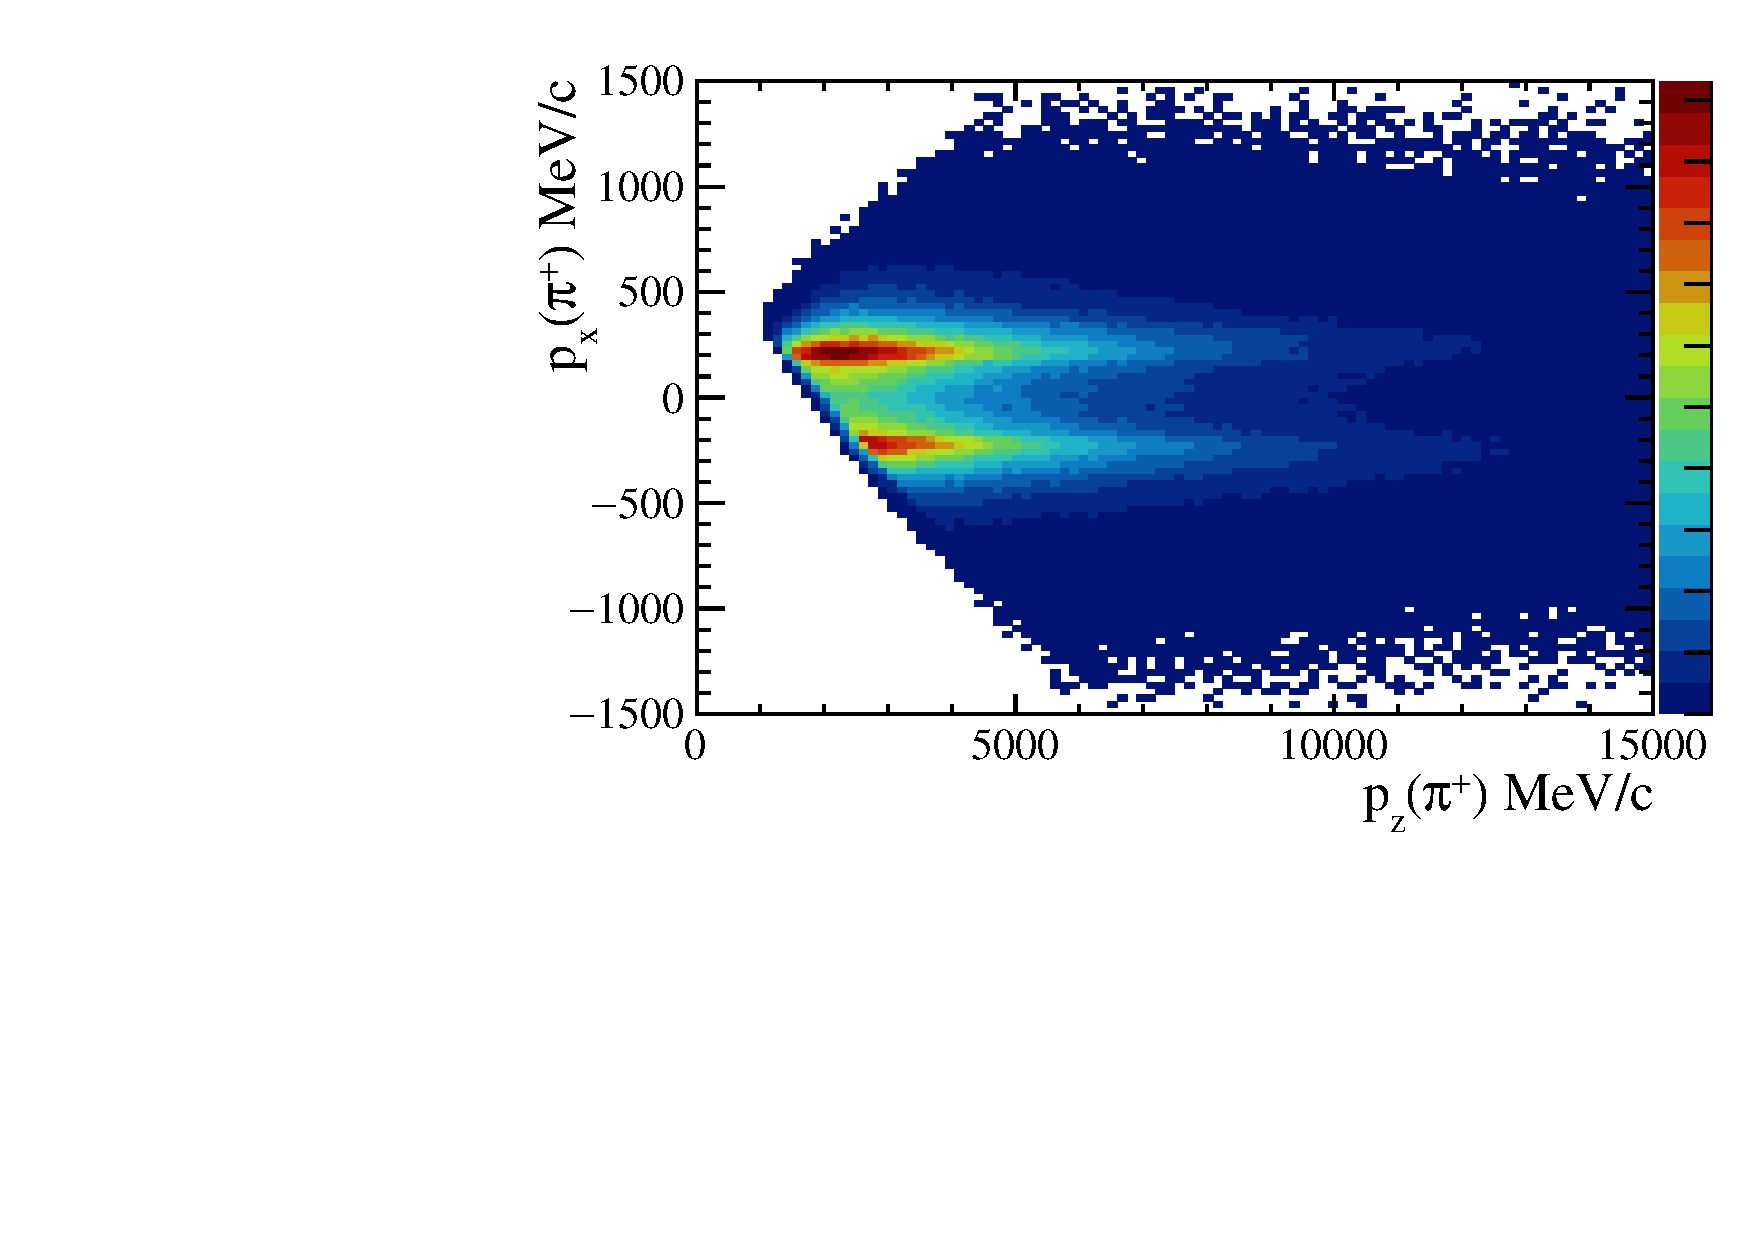
\includegraphics[width = 0.42\textwidth]{../work/RapidSimAnalysis/PGunAnalysis/Plots/KK_Dst_PXPZ_Positive.pdf}}
            \subfloat{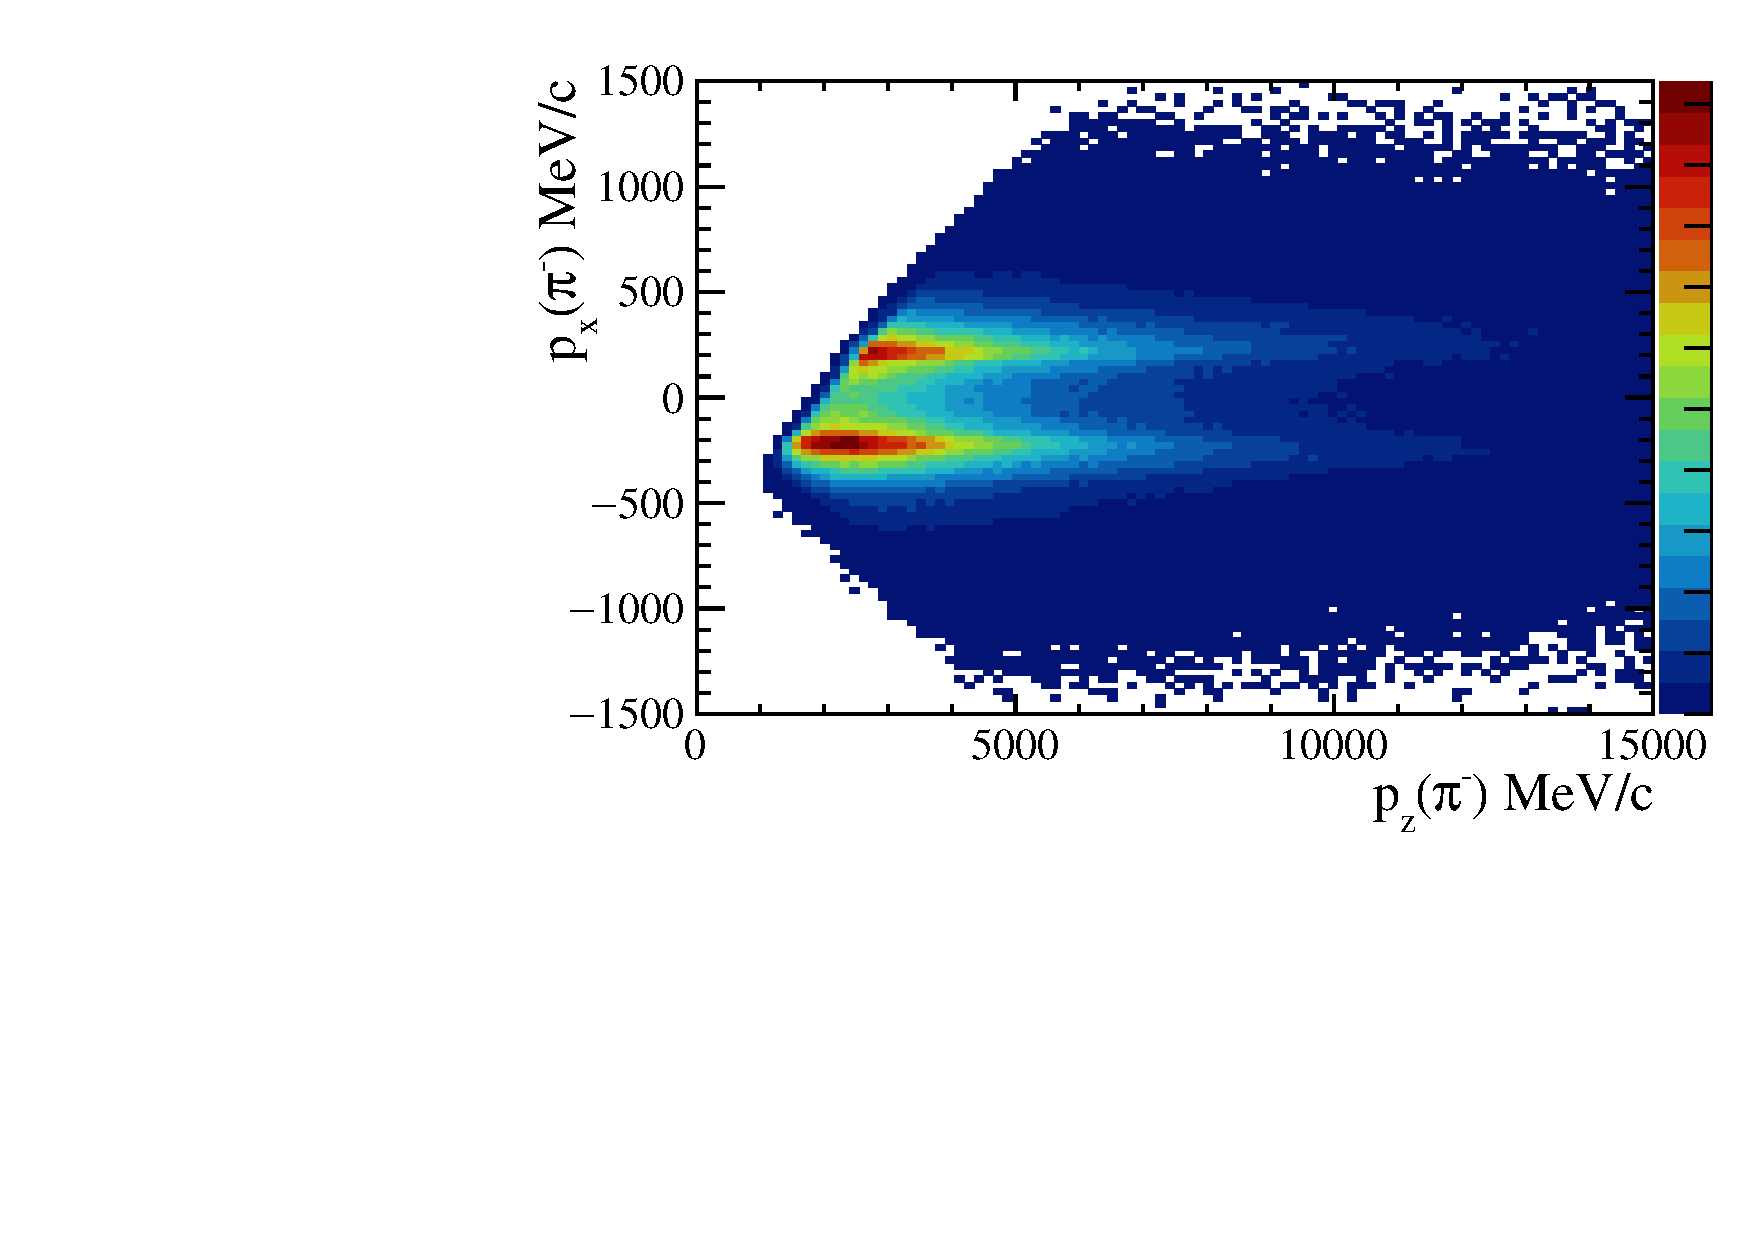
\includegraphics[width = 0.42\textwidth]{../work/RapidSimAnalysis/PGunAnalysis/Plots/KK_Dst_PXPZ_Negative.pdf}}
      \end{figure}
      \rightarrow The new weighting technique should yield $\Delta A_\text{total} = 0$
\end{frame}

\section{Conclusions}

\begin{frame}
      \LARGE
      \centering
      Thank you for your attention!

      Questions?
\end{frame}
\end{document}